\documentclass{article}
\usepackage[utf8]{inputenc}
\usepackage[spanish]{babel}
\usepackage{graphicx}
\usepackage{verbatim}
\usepackage{moreverb}
\usepackage{amsmath}
\usepackage{amsfonts}
\usepackage{amssymb}
\usepackage{fancybox}
\usepackage{float}
\usepackage{fancyvrb}
\usepackage{color}
\usepackage{hyperref}
\usepackage{multirow}


\usepackage{anysize}
\marginsize{1.5cm}{1.5cm}{1cm}{1cm}

\renewcommand{\shorthandsspanish}{}

\newcommand{\HRule}{\rule{\linewidth}{0.5mm}}

\begin{document}

\thispagestyle{empty}

%%%%%%%%%%%%%%%%%%%%%%%%%%%%%%%%% PORTADA %%%%%%%%%%%%%%%%%%%%%%%%%%%%%%%%%%%%%%

\begin{titlepage}
\begin{center}

%Espacio antes del logo del itba
\Large \  \\[1.5cm]


\includegraphics[scale=0.40]{Imagenes/logo_itba}\\[1cm]
\textsc{\LARGE Sistemas de inteligencia artificial}\\[1.5cm]
\textsc{\Large Trabajo práctico $\text{N}^{\circ}$3}\\[0.5cm]

\HRule \\[0.4cm]
{ \huge \bfseries Redes de Hopfield}\\[0.4cm]
\HRule \\[1.5cm]

\Large Autores: \\ [0.25cm]
\begin{tabular}{l @{\ \ -\ \ }l}
\Large Pablo Ballesty & \Large 49359\\[0.2cm]
\Large Nicolás Magni & \Large 48008\\[0.2cm]
\Large Guillermo Liss & \Large 49282 \\[0.2cm]
\end{tabular}



\vspace{1cm}

\vfill
% La fecha queda abajo.
{\large \today}

\end{center}
\end{titlepage}

%%%%%%%%%%%%%%%%%%%%%%%%%%%%%%%%%%%%%%%%%%%%%%%%%%%%%%%%%%%%%%%%%%%%%%%%%%%%%%%%

\abstract{
El objetivo del presente informe es detallar las decisiones tomadas durante el diseño e implementación de redes
de Hopfield, para ser utilizadas como memorias direccionables por el contenido. Como patrones se utilizan 25 imágenes
binarias provistas por la cátedra. Se presentan resultados y conclusiones obtenidas.
}

\section{Desarrollo}
En las siguientes secciones se detallan los aspectos que se consideraron destacables durante el desarrollo del trabajo.

\subsection{Evaluación y condición de corte}

Siguiendo el modelo de Hopfield la evaluación se realiza de forma asincrónica. Se asegura que luego de 4096 rondas,
todas las neuronas han actualizado su estado. De esta forma, se considera que el patrón de entrada convergió a un estado dado,
cuando las 4096 rondas arrojan el mismo resultado, llegado este punto se corta la evaluación.

\subsection{Estabilidad de patrones}
Para probar la estabilidad de los patrones almacenados en una red, se implementó un \emph{script} que calcula el \emph{crosstalk}
para cada posición del patrón. A continuación, se describe la regla para considerar a un patrón estable o inestable.


\begin{equation}
 \mbox{estable}(\xi^\mu) = \left\{ \begin{array}{ll}
 \mbox{\textbf{verdadero}} & \forall i \mbox{ crosstalk}(\xi^\mu_i) < 1 \\
  \mbox{\textbf{falso}} &\mbox{ en otro caso.}
       \end{array} \right.
\end{equation}

Luego, se utiliza esta regla para definir si un conjunto de patrones resulta estable o inestable. A continuación se presenta la misma.

\begin{equation}
 \mbox{conjuntoEstable}(\xi^{\mu_n}) = \left\{ \begin{array}{ll}
 \mbox{\textbf{verdadero}} & \forall n \mbox{ estable}(\xi^{\mu_n}) == \mbox{\textbf{verdadero}} \\
  \mbox{\textbf{falso}} &\mbox{ en otro caso.}
       \end{array} \right.
\end{equation}
Se entiende a $\xi^{\mu_n}$ como un conjunto finito de patrones $[\xi^{\mu_1} \xi^{\mu_2} \dots \xi^{\mu_n}]$ a almacenar.\\

De esta forma, si el conjunto de patrones almacenados resulta estable, se asegura que estos patrones son verdaderos
atractores de la red.


\subsection{Estados espurios}

Se desarrollaron dos \emph{scripts} diferentes, con el fin de generar patrones que puedan caer en cuencas de atracción de estados
espurios de la red. A continuación se describen los mismos:

\begin{itemize}
 \item \textbf{invert:} invierte el patrón que se le indica. Se utiliza con los patrones que se han almacenado en la red, a fin de
 observar si los patrones invertidos convergen a estados espurios de la red.
 \item \textbf{mixPatterns:} genera todas las posibles combinaciones lineales con coeficientes en 1 de los patrones que se le indican.
 A continuación se presenta la ecuación utilizada para definir el patrón mezcla, donde $\pm$ significa que se realizan 
 todas las posibles combinaciones de $+$ y $-$.
  \begin{equation}
    \forall i \;\; \xi^{\mbox{mix}}_{i} = \mbox{sign}(\pm \xi^{\mu_1}_i \pm \xi^{\mu_2}_i \dots \pm \xi^{\mu_n}_i)
  \end{equation}
\end{itemize}

\subsection{Remoción de estados espurios}

Se implementó un \emph{script} para intentar remover estados espurios que se encuentran al momento de evaluar
la red con diferentes patrones. El mismo, consiste en realizar los siguientes pasos:

\begin{enumerate}
 \item Se aplica a todos los pesos, el término corrector de la ecuación \ref{Eq:spu} siendo $S^f$ el estados espurio que se desea eliminar.
 \item Se evalúa el patrón que convergía a ese estado espurio, si este sigue convergiendo se vuelve al paso 1.
\end{enumerate}


\begin{equation}
  \label{Eq:spu}
   \Delta w_{ij} = -\dfrac{\epsilon}{N} S^{f}_{i} S^{f}_{j}
\end{equation}


\subsection{Cuencas de atracción}

Para analizar las cuencas de atracción de los patrones almacenados y los estados espurios en la red, se implementó
el \emph{script} \textbf{noise} el cual aplica ruido sobre el patrón indicado con una densidad $d$. Este mismo, se utiliza
en combinación con \textbf{invert} y \textbf{mixPatterns}, a fin de cubrir gran parte del dominio de entrada, y poder
analizar la convergencia en cada caso.


\subsection{Cantidad máxima de patrones almacenados}

Si se considera a un patrón como un conjunto de variables aleatorias independientes, donde la variable aleatoria puede tomar el valor 1 o -1 con igual
probabilidad. Se define $P_{\mbox{error}}$ como la probabilidad  de que un \emph{bit} elegido sea inestable. Esta puede estimarse, de la siguiente
forma

\begin{equation}
 P_{\mbox{error}} = \mbox{Prob}(C^{\nu}_i > 1).
\end{equation}
donde
\begin{equation}
 \label{eq:qty}
 C^{\nu}_i = -\xi^{\nu}_i \dfrac{1}{N} \sum_{j} \sum_{\mu \neq \nu} \xi^{\mu}_i \xi^{\mu}_j \xi^{\nu}_j.
\end{equation}
El término especificado en la ecuación \ref{eq:qty}, depende de $p$ (cantidad de patrones) y $N$ (cantidad de neuronas).
Si se consideran N y p grandes, por la ley de los grandes números, puede aproximarse la distribución binomial de $C^{\nu}_i$
como una distribución normal. Luego,

\begin{equation}
 P_{\mbox{error}} = \mbox{Prob}(C^{\nu}_i > 1) = \dfrac{1}{2}[1 - \mbox{erf}(\sqrt{N/2p})]
\end{equation}

donde

\begin{equation*}
 \mbox{erf}(x) = \dfrac{2}{\sqrt{\pi}} \int^x_0 \exp{(-u^2)}\delta u.
\end{equation*}

Luego, considerando aceptable un $P_{\mbox{error}} = 0.01$, se obtiene la relación $p_{\mbox{max}} = 0.15N$.
Por lo tanto, en nuestro caso como $N = 4096$, la cantidad máxima almacenable por la red es 

\begin{equation}
 p_{\mbox{max}} \simeq 614.
\end{equation}

Por lo tanto, teóricamente la red puede almacenar $614$ patrones. Sin embargo, los patrones que se poseen, no son un conjunto
de variables independietes, por lo que se implementó el \emph{script} \textbf{bestCombination} el cual busca el conjunto
más grande de patrones estables, con el fin de comparar la cantidad teórica y la cantidad real de patrones que se pueden
almacenar.

\section{Resultados}

\subsection{Prueba 1}

Para todas las pruebas en esta sección se utiliza una red que almacena los siguientes patrones

\begin{itemize}
 \item a.png
 \item line2.png
 \item windows.png
\end{itemize}
los mismos pueden verse en la figura \ref{Fig:stability}.

\subsubsection{Prueba de estabilidad}
Utilizando la regla \emph{conjuntoEstable} se obtiene que el conjunto de patrones resulta estable. Se evalúa
la red utilizando como entrada, los patrones almacenados. Se muestran los resultados obtenidos en la figura \ref{Fig:originals}.


\subsubsection{Prueba de atracción}
Para la misma red del caso anterior, se prueban como entrada los patrones almacenados pero con diferentes densidades
de ruido.

\begin{itemize}
 \item En la figura \ref{Fig:noise10} se presentan las entradas y los resultados obtenidos, habiendo aplicado un ruido con una densidad del 10\%.
 \item En la figura \ref{Fig:noise30} se presentan las entradas y los resultados obtenidos, habiendo aplicado un ruido con una densidad del 30\%.
 \item En la figura \ref{Fig:noise50} se presentan las entradas y los resultados obtenidos, habiendo aplicado un ruido con una densidad del 50\%.
\end{itemize}

También se prueban como entrada versiones incompletas de los patrones almacenados en la red. Se presentan los resultados obtenidos
en las figuras \ref{Fig:incomplete1} y \ref{Fig:incomplete2}.\\

Además, se prueban patrones que no fueron almacenados en la red. Se tomaron
\begin{itemize}
 \item h.png
 \item line1.png
 \item mac.png
\end{itemize}.
Se muestran los resultados en la figura \ref{Fig:others}.

\subsubsection{Prueba de patrones inversos}
Se prueban las salidas que arroja la red, para las entradas conformadas por los inversos de los patrones almacenados
en la red. Se muestran los resultados en la figura \ref{Fig:inverts}.

\subsubsection{Prueba de patrones mezcla}
Se prueban las salidas que arroja la red para entradas conformadas por mezclas de los patrones almacenados en la red.
Se muestran las entradas y los resultados en la figura \ref{Fig:mix}.

\subsubsection{Remoción de estados espurios}
Se intentan remover los estados espurios a los que llega la red, se pueden ver los resultados obtenidos
utilizando entradas inversas y mezcla de los patrones almacenados.
Luego de realizar los cambios en la red, se evalúan las entradas que convergían a esos estados, como también
los patrones originales.\\

En la figura \ref{Fig:spu1} se muestran los resultados obtenidos, luego de remover el estado conformado por 
el inverso del patrón \emph{a.png}.\\

En la figura \ref{Fig:spu2} se muestran los resultados obtenidos, luego de remover el estado conformado por la
mezcla de los patrones almacenados en la red.\\

\subsubsection{Prueba de energía}

En la figura \ref{Fig:energy}, se muestra el gráfico de la energía correspondiente a la evaluación de la entrada
\emph{a.png} con ruido del 50\%.

\subsection{Prueba 2}
Se utilizó el \emph{script} \textbf{bestCombination} para hallar el conjunto más grande de patrones estables. Se encontró
un conjunto conformado por los siguientes siete patrones

\begin{itemize}
 \item a.png
 \item bad-egg.png
 \item circle-union.png
 \item circle1.png
 \item footprint.png
 \item line1.png
 \item midnight-bsd.png.
\end{itemize}
En la figura \ref{Fig:bestCombination} se muestran los mismos.



\section{Conclusiones}

 \subsection{Memoria direccionable por el contenido}
 Se pudo observar que la red que almacena un conjunto de patrones estables funciona como una memoria direccionable por el contenido.
 En las figuras \ref{Fig:originals}, \ref{Fig:noise10}, \ref{Fig:noise30} y \ref{Fig:noise50} puede notarse que los patrones almacenados
 funcionan como verdaderos atractores, y estos poseen cuencas de atracción considerables.
 
 \subsection{Patrones atractores}
 Pudo notarse que además de existir los atractores correspondientes a los patrones almacenados en la red, existen otros atractores
 correspondientes a estados espurios. Puede verse en las figuras \ref{Fig:others}, \ref{Fig:inverts} y \ref{Fig:mix} que diferentes entradas
 convergen a estados espurios de la red.\\
 
 Se pudo notar, que los estados espurios correspondientes a los patrones almacenados invertidos poseen cuencas de atracción muy grandes
 y comparables con las de los patrones originales. Mientras que, los estados espurios conformados por la mezcla de patrones almacenados
 poseen una cuenca de atracción pequeña.
 
 \subsection{Eliminación de estados espurios}
 Se pudo notar que al eliminar estados espurios de la red se puede afectar también a los patrones almacenados. Puede verse en la figura 
 \ref{Fig:spu1} que al tratar de eliminar un estado espurio correspondiente al inverso de un patrón almacenado, luego si se utiliza
 el almacenado como entrada, ya no converge al atractor correspondiente.\\
 
 También se pudo observar en la figura \ref{Fig:spu2}, que al eliminar un estado espurio correspondiente a una mezcla de los patrones almacenados, también se elimina
 el estado espurio inverso.
 
 \subsection{Decrecimiento de la energía}
 Como era esperable, en la figura \ref{Fig:energy} se puede observar que en la evaluación la energía siempre decrece, que es lo correspondiente en
 un modelo de Hopfield, ya que las actualizaciones se realizan de forma asincrónica.
 
 \subsection{Capacidad de almacenamiento}
 Como se calculó, teóricamente la red puede almacenar como máximo 614 patrones distintos. Sin embargo, este cálculo está basado en que los patrones
 son un conjunto de variables aleatorias independientes. Se pudo notar que en la práctica la cantidad de patrones a almacenar depende de
 la similitud con respecto a la distancia de Hamming que poseen los patrones que se desean almacenar, y que la cantidad máxima es mucho menor
 a la calculada de forma teórica. En este caso, la cantidad máxima de patrones que se pudo almacenar fue de 7 patrones.
%  \color{red}
%  \begin{itemize}
%  \item Como era de esperar cuando los patrones son estables, cada uno converge a él mismo.
%  \item Se puede ver que un conjunto no estable, tiene problemas.
%  \item Es importante ver que los patrones son estables.
%  \item Se notó que los patrones inversos forman cuencas de atracción muy grandes. Y las comb. lineales re chicas.
%  \item Diferencia entre capacidad de almacenamiento teórica y real.
%  \item La capacidad depende de los patrones
%  \item Ver que el gráfico de la energía siempre decrece que es la idea.
% \end{itemize}


\clearpage

\appendix
\section{Imágenes}

\begin{center}

\begin{figure}[h!]
 \centering
 \fbox{
\includegraphics{../../src/img/original/a.png}}
 \fbox{
\includegraphics{../../src/img/original/line2.png}}
 \fbox{
\includegraphics[scale=1.34]{../../src/img/original/windows.png}}
 \caption{Patrones almacenados en la prueba de estabilidad}
 \label{Fig:stability}
\end{figure}
 
\begin{figure}[h!]
 \centering
 \fbox{
\includegraphics{../../src/img/original/a.png}}
 \fbox{
\includegraphics{../../src/img/original/a.png}}
 
 \fbox{
\includegraphics{../../src/img/original/line2.png}}
 \fbox{
\includegraphics{../../src/img/original/line2.png}}
 
 \fbox{
\includegraphics[scale=1.34]{../../src/img/original/windows.png}}
 \fbox{
\includegraphics[scale=1.34]{../../src/img/original/windows.png}}
 \caption{A la izquierda se presenta la entrada de la red, y a la derecha la salida obtenida.}
 \label{Fig:originals}
\end{figure}

\begin{figure}[h!]
 \centering
 \fbox{
\includegraphics{../../src/img/results/a_noise_10.png}}
 \fbox{
\includegraphics{../../src/img/original/a.png}}
 
 \fbox{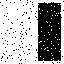
\includegraphics{../../src/img/results/line_noise_10.png}}
 \fbox{
\includegraphics{../../src/img/original/line2.png}}
 
 \fbox{
\includegraphics{../../src/img/results/win_noise_10.png}}
 \fbox{
\includegraphics[scale=1.34]{../../src/img/original/windows.png}}
 \caption{A la izquierda se presenta la entrada de la red, y a la derecha la salida obtenida.}
 \label{Fig:noise10}
\end{figure}

\begin{figure}[h!]
 \centering
 \fbox{
\includegraphics{../../src/img/results/a_noise_30.png}}
 \fbox{
\includegraphics{../../src/img/original/a.png}}
 
 \fbox{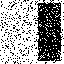
\includegraphics{../../src/img/results/line_noise_30.png}}
 \fbox{
\includegraphics{../../src/img/original/line2.png}}
 
 \fbox{
\includegraphics{../../src/img/results/win_noise_30.png}}
 \fbox{
\includegraphics[scale=1.34]{../../src/img/original/windows.png}}
 \caption{A la izquierda se presenta la entrada de la red, y a la derecha la salida obtenida.}
 \label{Fig:noise30}
\end{figure}

\begin{figure}[h!]
 \centering
 \fbox{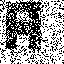
\includegraphics{../../src/img/results/a_noise_50.png}}
 \fbox{
\includegraphics{../../src/img/original/a.png}}
 
 \fbox{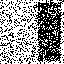
\includegraphics{../../src/img/results/line_noise_50.png}}
 \fbox{
\includegraphics{../../src/img/original/line2.png}}
 
 \fbox{
\includegraphics{../../src/img/results/win_noise_50.png}}
 \fbox{
\includegraphics[scale=1.34]{../../src/img/original/windows.png}}
 \caption{A la izquierda se presenta la entrada de la red, y a la derecha la salida obtenida.}
 \label{Fig:noise50}
\end{figure}

\begin{figure}[h!]
 \centering
 \fbox{
\includegraphics{../../src/img/tests/a_incomplete1.png}}
 \fbox{
\includegraphics{../../src/img/original/a.png}}
 
 \fbox{
\includegraphics{../../src/img/tests/line2_incomplete1.png}}
  \fbox{
\includegraphics{../../src/img/original/line2.png}}
 
 \fbox{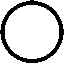
\includegraphics[scale=1.34]{../../src/img/tests/win_incomplete1.png}}
\fbox{
\includegraphics[scale=1.34]{../../src/img/original/windows.png}}
 \caption{A la izquierda se presenta la entrada de la red, y a la derecha la salida obtenida.}
 \label{Fig:incomplete1}
\end{figure}

\begin{figure}[h!]
 \centering
 \fbox{
\includegraphics{../../src/img/tests/a_incomplete2.png}}
 \fbox{
\includegraphics{../../src/img/original/a.png}}
 
 \fbox{
\includegraphics{../../src/img/tests/line2_incomplete2.png}}
 \fbox{
\includegraphics{../../src/img/original/line2.png}}

 \fbox{
\includegraphics[scale=1.34]{../../src/img/tests/win_incomplete2.png}}
 \fbox{
\includegraphics[scale=1.34]{../../src/img/original/windows.png}}
 \caption{A la izquierda se presenta la entrada de la red, y a la derecha la salida obtenida.}
 \label{Fig:incomplete2}
\end{figure}

\begin{figure}[h!]
 \centering
 \fbox{
\includegraphics{../../src/img/original/h.png}}
 \fbox{
\includegraphics{../../src/img/original/a.png}}
 
  \fbox{
\includegraphics{../../src/img/original/line1.png}}
 \fbox{
\includegraphics{../../src/img/original/a.png}}
 
 \fbox{
\includegraphics[scale=1.34]{../../src/img/original/mac.png}}
 \fbox{
\includegraphics{../../src/img/results/result_mac_windows.png}}
 \caption{A la izquierda se presenta la entrada de la red, y a la derecha la salida obtenida.}
 \label{Fig:others}
\end{figure}

\begin{figure}[h!]
 \centering
 \fbox{
\includegraphics{../../src/img/results/a_inv.png}}
 \fbox{
\includegraphics{../../src/img/results/a_inv.png}}
 
  \fbox{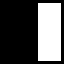
\includegraphics{../../src/img/results/line_inv.png}}
 \fbox{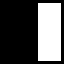
\includegraphics{../../src/img/results/line_inv.png}}
 
 \fbox{\includegraphics{../../src/img/results/win_inv.png}}
 \fbox{\includegraphics{../../src/img/results/win_inv.png}}
 \caption{A la izquierda se presenta la entrada de la red, y a la derecha la salida obtenida.}
 \label{Fig:inverts}
\end{figure}

\begin{figure}[h!]
 \centering
 \fbox{\includegraphics{../../src/img/results/mix1.png}}
 \fbox{\includegraphics{../../src/img/results/mix1.png}}
 
  \fbox{\includegraphics{../../src/img/results/mix2.png}}
 \fbox{\includegraphics{../../src/img/results/mix2.png}}

 \caption{A la izquierda se presenta la entrada de la red, y a la derecha la salida obtenida.}
 \label{Fig:mix}
\end{figure}

\begin{figure}[h!]
 \centering
 \fbox{\includegraphics{../../src/img/results/a_inv.png}}
 \fbox{\includegraphics{../../src/img/results/rem_spu_1.png}}
 
 \fbox{\includegraphics{../../src/img/original/a.png}}
 \fbox{\includegraphics{../../src/img/results/rem_spu_2.png}}

 \caption{A la izquierda se presenta la entrada de la red, y a la derecha la salida obtenida.}
 \label{Fig:spu1}
\end{figure}

\begin{figure}[h!]
 \centering
 \fbox{\includegraphics{../../src/img/results/mix1.png}}
 \fbox{\includegraphics{../../src/img/results/rem_spu_3.png}}
 
  \fbox{\includegraphics{../../src/img/results/mix2.png}}
 \fbox{\includegraphics{../../src/img/results/rem_spu_4.png}}

 \caption{A la izquierda se presenta la entrada de la red, y a la derecha la salida obtenida.}
 \label{Fig:spu2}
\end{figure}

\begin{figure}[h!]
 \centering
 \fbox{\includegraphics{../../src/img/results/a_noise_50.png}}
 \fbox{\includegraphics[scale=0.5]{../../src/img/results/energy_noise_50.png}}

 \caption{Energía en la evaluación de la entrada presentada a la izquierda.}
 \label{Fig:energy}
\end{figure}

\begin{figure}[h!]
 \centering
 \fbox{\includegraphics{../../src/img/original/a.png}}
 \fbox{\includegraphics{../../src/img/original/bad-egg.png}}
 \fbox{\includegraphics[scale=1.34]{../../src/img/original/circle-union.png}}
 
 \fbox{\includegraphics[scale=1.34]{../../src/img/original/circle1.png}}
 \fbox{\includegraphics[scale=1.34]{../../src/img/original/footprint.png}}
 \fbox{\includegraphics{../../src/img/original/line1.png}}
 \fbox{\includegraphics{../../src/img/original/midnight-bsd.png}}
 \caption{Conjunto de patrones estables más grande.}
 \label{Fig:bestCombination}
\end{figure}


\end{center}


\end{document}